% Date added: 2024/09/30

\subsection{The Carpet Cutting Problem}

This problem features a rather contrived example that only mathematicians would not question. I found this on the puzzles stack exchange, and most of the time that I spent solving it was used making a tool in Desmos to help test solutions. Once the tool was made, the logical solving path became much clearer, and I would recommend all trying to solve this to use the Desmos or a similar tool. Here is one I made (spoiler free): \url{https://www.desmos.com/calculator/clrourbpeo}.

A carpet is needed for a 7 metre by 10 metre room. There is a 6 metre by 1 metre section of carpet that cannot be cut, and an 8 metre by 8 metre square of carpet that can only be cut once. This cut can be as complicated as one desires, although cutting to the edge and then back in to the carpet again at the same point counts as two cuts and is not allowed. This includes diagonal, or even curved cuts.

\textbf{Hints:}

\begin{enumerate}
    \item The cut is symmetrical.
    \item The cut uses only orthogonal straight edges.
\end{enumerate}

\textbf{Solution:}

\begin{figure}[H]
	\begin{center}
		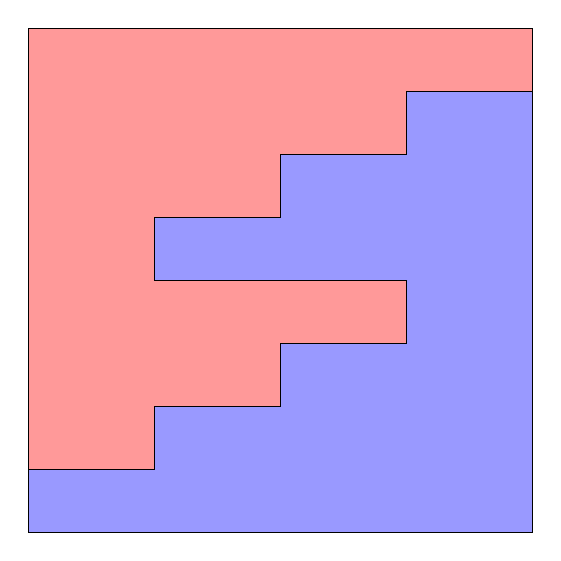
\begin{tikzpicture}[scale=0.8, baseline=(current bounding box.center)]
			
			\draw[black, fill=blue, fill opacity=0.4] (0, 0) -- (8, 0) -- (8, 7) -- (6, 7) -- (6, 6) -- (4, 6) -- (4, 5) -- (2, 5) -- (2, 4) -- (6, 4) -- (6, 3) -- (4, 3) -- (4, 2) -- (2, 2) -- (2, 1) -- (0, 1) -- (0, 0);
			\draw[black, fill=red, fill opacity=0.4] (8, 8) -- (8, 7) -- (6, 7) -- (6, 6) -- (4, 6) -- (4, 5) -- (2, 5) -- (2, 4) -- (6, 4) -- (6, 3) -- (4, 3) -- (4, 2) -- (2, 2) -- (2, 1) -- (0, 1) -- (0, 8) -- (8, 8);
			
		\end{tikzpicture}
		\hfill
		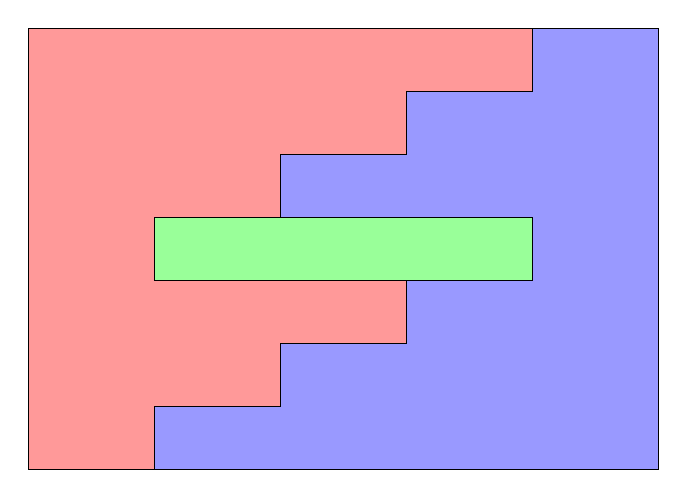
\begin{tikzpicture}[scale=0.8, baseline=(current bounding box.center)]
			
			\draw[black, fill=blue, fill opacity=0.4] (2, 1) -- (10, 1) -- (10, 8) -- (8, 8) -- (8, 7) -- (6, 7) -- (6, 6) -- (4, 6) -- (4, 5) -- (8, 5) -- (8, 4) -- (6, 4) -- (6, 3) -- (4, 3) -- (4, 2) -- (2, 2) -- (2, 1);
			\draw[black, fill=red, fill opacity=0.4] (8, 8) -- (8, 7) -- (6, 7) -- (6, 6) -- (4, 6) -- (4, 5) -- (2, 5) -- (2, 4) -- (6, 4) -- (6, 3) -- (4, 3) -- (4, 2) -- (2, 2) -- (2, 1) -- (0, 1) -- (0, 8) -- (8, 8);
			\draw[black, fill=green, fill opacity=0.4] (2, 4) -- (8, 4) -- (8, 5) -- (2, 5) -- (2, 4);
			
		\end{tikzpicture}
	\end{center}
\end{figure}

\textbf{Extensions and Comments:}

